% Drawing 138/06-12 -- folder 138, batch 06, archive page 108 (PDF page 109).
% Transcription: un hexagone, sommets marqués $0$ et $1$, avec des traits qui en partent ; à côté, « $\widetilde{X}$ » et « $\underline{a}$ ».
% Kind: hexagon with strokes. Method 2 (schematic redraw from the facsimile). Status: partial.
% Notes: A hexagon (ink), every side drawn between the same six vertex points; the vertices 0 (bottom) and 1 (right) labelled; the left side doubled (drawn thick). From the left vertex: four thin strokes (two up, two down) and a long thin stroke crossing the upper left side; from the vertex 0: two nearly parallel pencil strokes up into the hexagon (a narrow lens) and a thin stroke down; inside the hexagon in pencil: a short curved stroke right of the lens, two near-vertical strokes left of the middle of the upper side (one with a short dark tick), a small arc on the second of them and a short stroke beside it. The bbox is widened to the left so that the strokes at the left vertex are whole. Second pass 2026-11-14 (issue 147, Claude Opus 5.5): the pencil strokes inside the hexagon that the scan shows clearly (the two strokes from the vertex 0, the curved stroke beside them, the two near-vertical strokes on the right with their tick, arc and short stroke) drawn stroke by stroke from a high-contrast grid overlay at 28 px per unit; laid over the crop they lie on their pencil to within about half a unit, the hexagon within about half a unit. Still differs: the faint diagonal pencil hatching across the interior (some ten very faint parallel strokes from lower left to upper right) is left out, too faint at 250 ppi to place stroke by stroke; where the strokes leaving the left vertex end under the formulas is a reading. Not on the crop: the « X~ » and « a » are isolated text below and to the right of the hexagon, not drawn. The formulas crossing the figure are text. Nothing is struck. Not compiled (no TeX engine in the session).
% Coordinates: 1 unit = 1 mm = 1/100 of the crop width (bbox in page fractions: [0.22, 0.13, 0.58, 0.31]).
% Redrawn by Claude (claude-opus-5-5), issue #73, 2026-11-09; not checked by a human; not compiled (no TeX in the session).
% Checked by Claude (claude-opus-5-5) 2026-11-14 (issue #147, second pass): strokes redrawn from the 300 dpi colour render of the 250 ppi scan, coordinates read on a grid overlay and checked by overlaying the rasterised redraw; not compiled (no TeX in the session). Not checked by a human. Status: partial.
% Rights: reproduces part of the work -- behind RENDER_TRANSCRIPTS, never published by itself.
\documentclass[tikz,border=3pt]{standalone}
\usepackage{amsmath,amssymb}
\usetikzlibrary{patterns,arrows.meta}
\tikzset{pencil/.style={black!45}, struck/.style={black!35}, mark/.style={circle,draw,inner sep=1.3pt}, pt/.style={circle,fill,inner sep=0.9pt}, opt/.style={circle,draw,fill=white,inner sep=1.1pt}}
\begin{document}
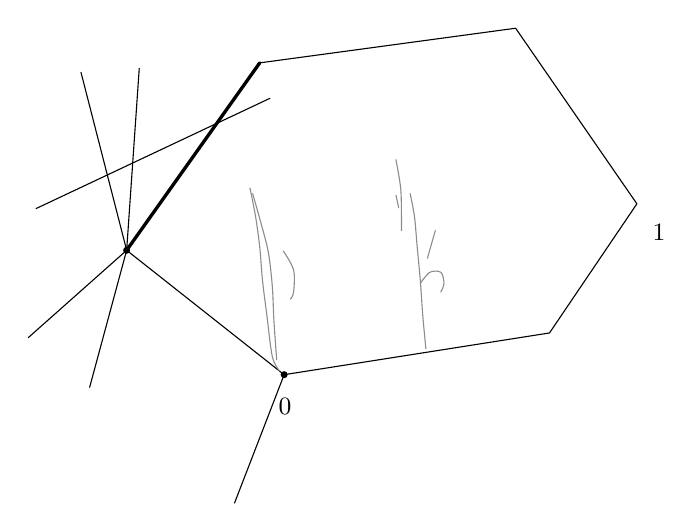
\begin{tikzpicture}[x=1mm,y=1mm,line cap=round,line join=round,font=\scriptsize]
\draw (42.1,-14.6) -- (74.6,-10.2) -- (90,-32.5) -- (78.9,-48.9) -- (45.2,-54.2) -- (25.2,-38.4) -- cycle;
\draw[very thick] (25.2,-38.4) -- (42.1,-14.6);
\draw (25.2,-38.4) -- (19.4,-15.8);
\draw (25.2,-38.4) -- (26.8,-15.3);
\draw (25.2,-38.4) -- (20.5,-55.8);
\draw (25.2,-38.4) -- (12.7,-49.5);
\draw (13.7,-33.1) -- (43.4,-19.1);
\draw[pencil] plot[smooth, tension=0.55] coordinates {(40.86,-30.5) (41.57,-34.1) (42.1,-38) (42.46,-42.3) (43,-46.6) (43.7,-51.9) (44.6,-53.7)};
\draw[pencil] plot[smooth, tension=0.55] coordinates {(41.2,-31.2) (42.3,-35.1) (43.2,-38.7) (43.7,-43) (43.9,-47.3) (44.25,-52.3)};
\draw[pencil] plot[smooth, tension=0.55] coordinates {(45.1,-38.5) (46.4,-40.9) (46.4,-43.7) (46,-44.6)};
\draw[pencil] plot[smooth, tension=0.55] coordinates {(59.4,-26.9) (60,-30.5) (60.1,-34) (60.1,-35.9)};
\draw[pencil] (59.4,-31.4) -- (59.75,-33);
\draw[pencil] plot[smooth, tension=0.55] coordinates {(61.2,-31.2) (61.75,-34.1) (62.1,-38) (62.5,-42.3) (62.8,-46.6) (63.2,-50.9)};
\draw[pencil] plot[smooth, tension=0.55] coordinates {(62.5,-42.6) (63.7,-41.2) (65.1,-41.2) (65.5,-42.6) (65.1,-43.7)};
\draw[pencil] (64.4,-35.9) -- (63.4,-39.4);
\draw (45.2,-54.2) -- (38.9,-70.5);
\node[pt] at (45.2,-54.2) {};
\node[pt] at (25.2,-38.4) {};
\node[inner sep=1pt] at (45.3,-58.2) {\small $0$};
\node[inner sep=1pt] at (92.8,-36.1) {\small $1$};
\end{tikzpicture}
\end{document}
